\chapter{Humanoids and steerable WMRs}
\label{ch:humanoids-and-swmrs}
The idea of building a machine that replicates the human body, and is capable 
of executing the same tasks that we do, has fascinated humanity since forever.
The earliest ideas can be dated back to the third century BC, when the 
Chinese philosopher Lie Yokou described a humanoid automaton constructed of 
leather and wood, capable of moving all parts of its body
\cite{Needham1956ScienceandCivilisationinChinaVol2}. In the first century AD,
the greek mathematician and engineer Heron of Alexandria described a machine 
capable of pouring wine for party guests \cite{Alexandria2015Pneumatica}.
In 1206, the Muslim engineer Ismail al-Jazari published a book describing 
about one hundred mechanical devices, including automata performing different 
facial expressions \cite{AlJarari1206BookofKnowledge}. Among these ancient
automata, the most famous one is undoubtedly Leonardo's mechanical knight 
(or Leonardo's robot), a humanoid automaton in a suit of a knight's armor
build by Leonardo Da Vinci in 1495 \cite{Moran2006TheDaVinciRobot}.
Even though the history of robots started many centuries ago, the word ``robot''
first appears only in 1920 in the science-fiction play R.U.R.
(Rossum's Universal Robots) \cite{Capek1920RUR}, written by the Czech writer
Karel {\v C}apek.
In the last century, robots have become part of our world. Apart the adoption 
of robots in the industry, and the use of robots in academia, we are now 
used to see robots in movies (e.g., C-3PO in Star Wars,
Fig. \ref{fig:introduction:robots-in-history}), in animation (e.g., The Iron
Giatn, Bender and Baymax, Fig.
\ref{fig:introduction:robots-in-animation}), and in books (Isaac Asimov
introduced the Three Laws of Robotics in his 1942 ``Runaround'' story).

This chapter gives a brief overview on the main developments in the field of 
robotics happened in the last 50 years, focusing in particular on humanoids
(from the WABOT-1 to the commercialization of humanoids)
and steerable WMRs (from interaction with humans to space exploration),
which are the type of platforms used in the following chapters.

\begin{figure}
    \centering
    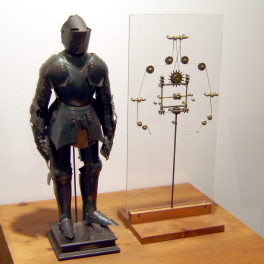
\includegraphics[width=\textwidth]{figures/01-introduction/robot-history.jpg}
    \caption{From left to right: Leonardo's robot, constructed by Leonardo Da
        Vinci in 1495 \cite{Moran2006TheDaVinciRobot};
        R.U.R. (Rossum's Universal Robots) by Karel {\v C}apek introduced 
        the word ``robot'' in 1920 \cite{Capek1920RUR};
        C-3PO, the famous humanoid robot from the Star Wars Cinematic Universe
        \cite{StarWars1977}.
    }
    \label{fig:introduction:robots-in-history}
\end{figure}

\begin{figure}
    \centering
    
\includegraphics[width=\textwidth]{figures/01-introduction/robots-in-animation.jpg}
    \caption{Humanoid robots in animation. From left to right:
        The Iron Giant (1999) \cite{TheIronGiant1999},
        Bender from Futurama (1999) \cite{Futurama1999}, and
        Baymax from Big Hero 6 (2014) \cite{BigHero62014}.
    }
    \label{fig:introduction:robots-in-animation}
\end{figure}

\subsubsection{First prototypes: WABOT-1 and WABOT-2}
The first anthropomorphic robot ever developed is the WABOT-1
\cite{Kato1973TheWABOT1}, whose project started in 1967 and completed in 1972.
The robot (Fig. \ref{fig:introduction:WABOTs}), was constituted by a limb-control
system, which allowed it to walk, and a conversation system, 
which allowed it to communicate with a person in Japanese. The development 
continued with the WABOT-2 \cite{Kato1987WABOT2}, introduced in 1984,
a musician robot able to play a keyboard instrument (Fig.
\ref{fig:introduction:WABOTs}) and read a musical score with his eyes. The WABOT
project is considered as a turning-point in the development of humanoids, as it 
introduced the first programmable multi-purpose humanoid robot.

\begin{figure}
    \centering
    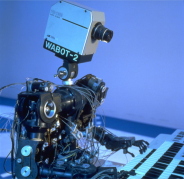
\includegraphics[width=0.7\textwidth]{figures/01-introduction/WABOTs.jpg}
    \caption{From left to right: the WABOT-1 (1972), which is the first anthropomorphic robot
        ever developed \cite{Kato1973TheWABOT1}, and the WABOT-2 (1984)
        playing a keyboard \cite{Kato1987WABOT2}.}
    \label{fig:introduction:WABOTs}
\end{figure}

\subsubsection{Honda humanoids: E series, P series and ASIMO}
\begin{figure}
    \centering
    \includegraphics[width=0.7\textwidth]{figures/01-introduction/The-ASIMO-humanoid-robot-history.png}
    \caption{Honda E series (E0 in 1986 to E6 in 1993) robots, Honda P series (P1 in
        1993 to P3 in 1997) robots, and ASIMO (2000)
        \cite{Shigemi2019ASIMOandHumanoidRobotResearchatHonda}.}
    \label{fig:introduction:ASIMO-humanoid-history}
\end{figure}

\subsubsection{2000s: humanoid robots play soccer}
\begin{figure}
    \centering
    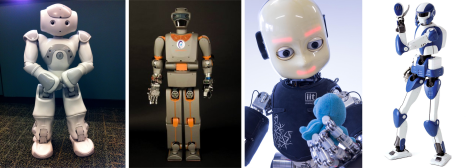
\includegraphics[width=\textwidth]{figures/01-introduction/robots-in-2000.jpg}
    \caption{Some of the humanoid robots developed in 2000s. From left to right:
        Aldebaran NAO \cite{Gouaillier2008NAOHumanoid},
        PAL Robotics REEM-B \cite{Tellez2008REEMB},
        iCub \cite{Metta2010iCubHumanoid}, and
        HRP-4 \cite{Kaneko2011HRP4}.
    }
    \label{fig:introduction:robots-in-2000}
\end{figure}

\subsubsection{2010s: DARPA robotics challenge}
\begin{figure}
    \centering
    \includegraphics[width=\textwidth]{figures/01-introduction/robots-in-2010.jpg}
    \caption{Some of the humanoid robots developed in 2010s. From left to right:
        Boston Dynamics ATLAS,
        WALK-MAN \cite{Tsagarakis2017WALKMAN},
        NASA Valkyrie \cite{Radford2015Valkyrie}, and
        PAL Robotics TALOS \cite{Stasse2017TALOS}.}
    \label{fig:introduction:robots-in-2010}
\end{figure}

\subsubsection{2020s: humanoids as commercial products}
\begin{figure}
    \centering
    \includegraphics[width=\textwidth]{figures/01-introduction/robots-in-2020.jpg}
    \caption{Some of the humanoid robots developed in 2020s for commercial
        purposes. From left to right:
        Digit by Agility Robotics, Optimus by Tesla, Apollo by Apptronik, and
        Figure 01 by Figure AI.
    }
    \label{fig:introduction:robots-in-2020}
\end{figure}

\subsubsection{Steerable WMRs: space exploration, disaster response, human collaboration}
\begin{figure}
    \centering
    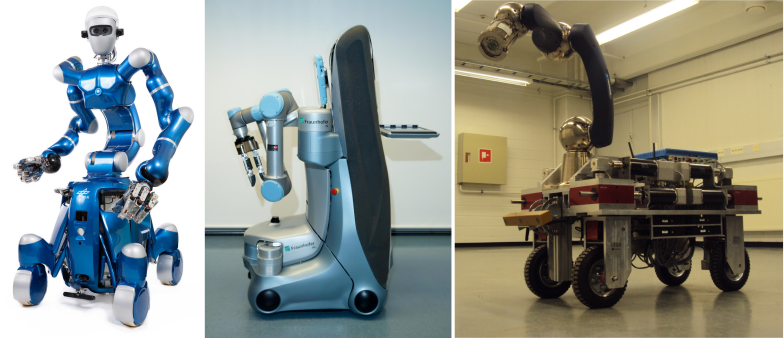
\includegraphics[width=\textwidth]{figures/01-introduction/SWMRs-1.jpg}
    \caption{Robots equipped with steerable wheels to be deployed in different areas.
        From left to right: Rollin' Justin \cite{Fuchs2009RollinJustin}, used 
        for household work and astronauts assistance in space, 
        Care-O-bot 3 \cite{Graf2009Care-O-bot3}, used as service robot, and
        iMoro \cite{Oftadeh2013iMoro}, used for inspection of contaminated
        environments.}
    \label{fig:introduction:SWMRs-1}
\end{figure}

\begin{figure}
    \centering
    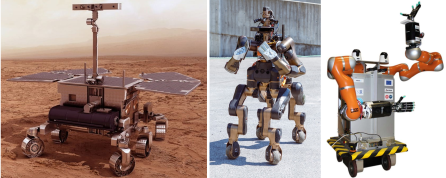
\includegraphics[width=\textwidth]{figures/01-introduction/SWMRs-2.jpg}
    \caption{More recent robots equipped with steerable wheels.
        ExoMars \cite{Poulakis2015ExoMarsMobilitySubsystem}, conceived for 
        space exploration,
        CENTAURO \cite{Kashiri2019Centauro}, designed for loco-manipulation
        in disaster scenarios, and
        BAZAR \cite{Cherubini2019ACR}, designed to interact with humans in
        assembly lines.
    }
    \label{fig:introduction:SWMRs-2}
\end{figure}
